%--------------------------------------------------------------------------------
% CONFIGURATION DU DOCUMENT
%--------------------------------------------------------------------------------

\documentclass[a4paper,12pt]{report}

\usepackage[french]{babel}
\usepackage[utf8]{inputenc}
\usepackage[T1]{fontenc}
\usepackage{mathptmx}
\usepackage[most]{tcolorbox}
\usepackage[a4paper, left=2.5cm, right=2.5cm, top=2.5cm, bottom=2.5cm]{geometry}
\usepackage{graphicx}
\usepackage{lipsum}
\usepackage{hyperref}
\usepackage{amsmath, amssymb}
\usepackage{float}

\usepackage{pgfplots}
\usepackage{tikz} 
\usetikzlibrary{shapes.geometric, trees, arrows, arrows.meta}

\setlength{\textfloatsep}{10pt}

\begin{document}





%--------------------------------------------------------------------------------
% PAGE DE GARDE
%--------------------------------------------------------------------------------

\begin{titlepage}
    \centering

    %----------------------------------
    % Informations sur l'université
    %----------------------------------

    {\large Faculté des Sciences et Ingénierie - Sorbonne Université}\\[0.3cm]
    {\large Master Informatique parcours ANDROIDE}\\[1cm]
    
\includegraphics[width=0.3\textwidth]{../images/logo_SU.png}\\[1.5cm]


    %----------------------------------
    % Informations sur le projet
    %----------------------------------

    \vspace{1.5cm}

    {\LARGE COMPLEX - Complexité, algorithmes randomisés et approchés}\\[1cm]
    {\Large Rapport de projet}\\[2cm]
    \rule{\linewidth}{0.5mm} \\[1cm]
    {\Huge \textbf{Arbres Cartésien et Algorithmes associés}} \\[0.4cm]
    \rule{\linewidth}{0.5mm} \\[2cm]
    

    %----------------------------------
    % Informations sur nous
    %----------------------------------

    \begin{flushleft}
        \textbf{Réalisé par :} \\[0.3cm]
        PINHO FERNANDES Enzo \\[0.2cm]
        BEN SALAH Adel \\[2cm]
    \end{flushleft}
    

    %----------------------------------
    % Date
    %----------------------------------

    \vfill
    {\large Novembre 2024}\\
    
\end{titlepage}





%--------------------------------------------------------------------------------
% Table des matières
%--------------------------------------------------------------------------------

\tableofcontents





%--------------------------------------------------------------------------------
% Page d'introduction
%--------------------------------------------------------------------------------

\newpage

\chapter*{Introduction du projet}
\addcontentsline{toc}{chapter}{Introduction du projet}

Les arbres cartésiens sont une structure de données qui combine les propriétés des arbres binaires de recherche et des tas. Ils ont été proposés par Jean 
    Vuillemin en 1980. Voici un aperçu de leur structure et de leur fonctionnement :\\[-0.4cm]


\textbf{Structure}
\begin{itemize}

    \item \textbf{Noeuds :} chaque noeud d'un arbre cartésien contient une clé (qui respecte l'ordre d'un arbre binaire de recherche) 
        et une priorité (qui respecte l'ordre d'un tas).

    \item \textbf{Arbre binaire de recherche :} les noeuds sont organisés de manière à ce que, pour tout noeud, les clés de son 
        sous-arbre gauche soient inférieures à sa clé, et celles de son sous-arbre droit soient supérieures.

    \item \textbf{Tas :} les noeuds sont également organisés selon la priorité, de sorte qu'un parent ait toujours une priorité inférieure 
        à celle de ses enfants.

\end{itemize}


\begin{figure}[!h]
    \centering
    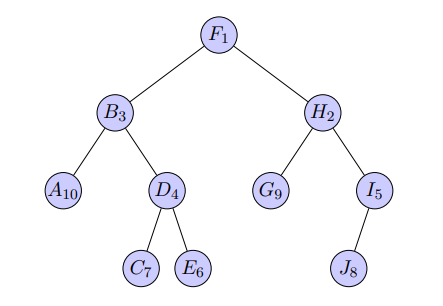
\includegraphics[width=0.5\textwidth]{../images/figure1.png}
    \caption{Exemple d'arbre cartésien contenant les clés de \{A,B,\dots,J\} avec les valeurs de priorités dans \{1,\dots,10\} données en indice.}
\end{figure}


\textbf{Propriétés}
\begin{itemize}

    \item \textbf{Équilibre probabiliste :} Les arbres cartésiens maintiennent une structure équilibrée de manière \textbf{probabiliste}. 
        Cela signifie que les opérations d'insertion, de suppression et de recherche ont une complexité en temps moyenne de \( O(\log n) \) même si 
        dans le pire des cas, cela peut atteindre \( O(n) \) (où \( n \) désigne le nombre de noeuds de l'arbre cartésien).

    \item \textbf{Insertion et suppression :} Lors de l'insertion, un nouveau noeud est placé comme un noeud feuille dans l'arbre binaire 
        de recherche. Puis, si sa priorité est inférieure à celle de son parent, il est "élevé" à travers des rotations jusqu'à ce que l'ordre du tas soit 
        respecté (\textit{cf.} Exercice 3).

    \item \textbf{Recherche :} La recherche d'une clé suit les règles d'un arbre binaire de recherche, ce qui la rend efficace.

\end{itemize}


\newpage

Les arbres cartésiens sont utilisés dans diverses applications où une structure de données dynamique et équilibrée est nécessaire, comme la gestion de 
    fichiers, les bases de données et les algorithmes de traitement d'événements. Le but de ce projet est d'implanter et d'analyser cette structure de 
    données et d'effectuer des tests d'efficacités.





%--------------------------------------------------------------------------------
% Exercice 1 : Arbres cartésiens - Premières propriétés
%--------------------------------------------------------------------------------

\newpage

\renewcommand{\chaptername}{Exercice}
\chapter{Arbres cartésiens - Premières propriétés}



%--------------------------------------------------------------------------------
% Question 1.a
%--------------------------------------------------------------------------------

\addcontentsline{toc}{section}{a. Construction de l'arbre cartésien}

\textbf{1.a]} Construire un arbre cartésien dont les noeuds sont donnés par la liste suivante (la lettre représentant la clé du noeud et l'entier sa priorité) :
\[
(A:5), (B:3), (C:8), (D:2), (E:6), (F:7), (G:9), (H:1), (I:10), (J:12)
\]
Existe-t-il plusieurs solutions ? Qu'en est-il pour un arbre cartésien dont toutes les priorités sont différentes (ce que nous ferons dans toute la suite du projet). 
    Justifier votre réponse.\\



\begin{tcolorbox}[colback=gray!10, colframe=blue!30, coltitle=black, title=Réponse à la 1.a - 1/2]
    
    Arbre cartésien de la liste précédente :\\


    % Arbre cartésien de la question Q1.a
    \begin{center}
        \begin{tikzpicture}[every node/.style = {minimum width = 2em, draw, circle}, level/.style = {sibling distance = 50mm/#1}]
            \node {\(H_1\)}
            child {   
                node {\(D_2\)} 
                child {   
                    node {\(B_3\)}
                    child {
                        node {\(A_5\)}
                    }
                    child {
                        node {\(C_8\)}
                    }
                }
                child {
                    node {\(E_6\)}
                    child {edge from parent[draw = none]}
                    child {
                        node {\(F_7\)}
                        child {edge from parent[draw = none]}
                        child {
                            node {\(G _9\)}
                        }
                    }
                }
            }
            child {
                node {\(I_{10}\)}
                child {edge from parent[draw = none]}
                child {
                    node {\(J_{12}\)}
                }
            };
        \end{tikzpicture}
    \end{center}


    Il n'existe pas plusieurs solutions, et cela est vrai également pour tout arbre cartésien dont toutes les priorités sont différentes, grâce aux 
        propriétés d'un arbre de recherche binaire et d'un tas.


    \vspace{0.5cm}
    \hrule
    \vspace{0.5cm}


    En effet, dans un arbre cartésien, la \textbf{racine} doit être le noeud avec \textbf{la priorité la plus faible} parmi tous les noeuds par la propriété 
        du tas. Par conséquent, il n'y a qu'une possibilité, le choix de la racine est unique.


\end{tcolorbox}
\begin{tcolorbox}[colback=gray!10, colframe=blue!30, coltitle=black, title=Réponse à la 1.a - 2/2]


    Une fois cela fait, l'ensemble des autres noeuds de priorité inférieure seront divisés en deux sous-ensembles selon leur clé, d'après la propriété d'un 
        arbre de recherche binaire :\\[-0.4cm]
    \begin{itemize}
        \item Le sous-arbre gauche contiendra tous les noeuds ayant des clés inférieures à celle de la racine.
        \item Le sous-arbre droit contiendra tous les noeuds ayant des clés supérieures à celle de la racine.
    \end{itemize}


    \vspace{0.5cm}

    Ces deux sous-ensembles sont indépendants l'un de l'autre, et surtout uniques. Chacun de ces sous-ensembles doivent représenter eux-même un arbre cartésien.\\

    On suivra le même raisonnement récursivement sur les sous-ensembles gauche et droit :\\[-0.4cm]
    \begin{itemize}
        \item On choisit le noeud du premier sous-ensemble avec la priorité la plus faible comme racine.
        \item On choisit le noeud du second sous-ensemble avec la priorité la plus faible comme racine.
    \end{itemize}

    \vspace{0.5cm}

    Et on recommence jusqu'à que tous les noeuds soient placés dans l'arbre cartésien.


    \vspace{0.5cm}
    \hrule
    \vspace{0.5cm}


    En conclusion, \textbf{tout arbre cartésien est unique} (si toutes les priorités sont différentes) puisque chaque décision de construction 
        est unique, alias :\\[-0.4cm]
    \begin{itemize}
        \item Le choix de la racine, de par sa priorité la plus faible de son sous-ensemble, grâce à la propriété du tas.
        \item Le choix des deux sous-ensembles, de par les clés des noeuds, grâce à la propriété des arbres de recherche binaire. 
    \end{itemize}

\end{tcolorbox}



%--------------------------------------------------------------------------------
% Question 1.b
%--------------------------------------------------------------------------------

\newpage
\addcontentsline{toc}{section}{b. Insertion de noeuds dans un ordre prédéfini}

\textbf{1.b]} Considérer l'arbre binaire de recherche construit en insérant dans l'ordre les noeuds dont les clés sont les suivantes : \( H, D, B, A, E, F, C, G, I \) et \( J \) et comparer à l'arbre cartésien de la question précédente. Généraliser et démontrer ce résultat pour un arbre cartésien général (dont les priorités sont différentes).\\



\begin{tcolorbox}[colback=gray!10, colframe=blue!30, coltitle=black, title=Réponse à la 1.b - 1/1]

    L'arbre issu de l'insertion de ces noeuds, dans cet ordre, donne exactement le même arbre cartésien de la question précédente.\\

    \begin{center}
        \begin{tikzpicture}[every node/.style = {minimum width = 2em, draw, circle}, level/.style = {sibling distance = 50mm/#1}]
            \node {\(H\)}
            child {   
                node {\(D\)} 
                child {   
                    node {\(B\)}
                    child {
                        node {\(A\)}
                    }
                    child {
                        node {\(C\)}
                    }
                }
                child {
                    node {\(E\)}
                    child {edge from parent[draw = none]}
                    child {
                        node {\(F\)}
                        child {edge from parent[draw = none]}
                        child {
                            node {\(G \)}
                        }
                    }
                }
            }
            child {
                node {\(I\)}
                child {edge from parent[draw = none]}
                child {
                    node {\(J\)}
                }
            };
        \end{tikzpicture}
    \end{center}

    Nous avons cette corrélation entre les deux arbres parce que nous avons inséré les noeuds selon leur priorité (en ordre croissant) dans l'arbre cartésien.

    \vspace{0.5cm}
    \hrule
    \vspace{0.5cm}

    On peut généraliser ce résultat en : un arbre cartésien est un ABR où nous avons inséré les noeuds dans l'ordre croissant de leur priorité (si elles sont toutes différentes).\\

    En effet, trois propriétés sont visibles dans ce cas précis :\\[-0.4cm]
    \begin{itemize}
        \item La racine des deux arbres sont les mêmes, alias le noeud dont la priorité est la plus faible.
        \item La propriété de l'ABR est respecté dans les deux cas, étant donné la nature des arbres.
        \item La propriété du tas est respecté pour l'arbre cartésien bien évidemment, mais également pour cet ABR. En effet, pour ce dernier, 
            on insère les noeuds dans l'ordre croissant de leur priorité. D'après l'algorithme d'insertion de ce dernier, il deviendra forcément une des 
            feuilles de l'arbre à la fin de l'insertion, et il n'y a pas de rotation. Par conséquent, tout parent de cet arbre aura une priorité plus 
            faible que leurs enfants.
    \end{itemize}

    \vspace{0.5cm}

    Étant donné que tout arbre respectant les propriétés d'un ABR et d'un tas est unique, et que dans ce cas précis, nos deux arbres respectent ces 
        propriétés et possèdent la même racine, alors... Ils sont égaux, dû à leur unicité.

\end{tcolorbox}



%--------------------------------------------------------------------------------
% Question 1.c
%--------------------------------------------------------------------------------

\newpage
\addcontentsline{toc}{section}{c. Implantation de la structure de données d'un noeud}

\textbf{1.c]} Programmer la structure de données d'un noeud (contenant la clé et la priorité, le pointeur vers le fils gauche, le pointeur vers le fils droit) 
    avec les constructeurs et les fonctions associés.



\begin{tcolorbox}[colback=gray!10, colframe=blue!30, coltitle=black, title=Réponse à la 1.c - 1/1]

    Nous avons décidé d'implémenter nos différentes structures de données en JAVA, pour sa simplicité quant à l'utilisateur des pointeurs ainsi que de la mémoire.\\

    En effet, le garbage collector s'occupe de libérer la mémoire dès qu'un objet n'est plus référencé, ce qui nous sera très pratique au moment de la 
        suppression des noeuds.\\

    L'Implantation se trouve dans le fichier : \href{./src/Node.java}{./src/Node.java}

\end{tcolorbox}



%--------------------------------------------------------------------------------
% Question 1.d
%--------------------------------------------------------------------------------

\vspace{1.5cm}
\addcontentsline{toc}{section}{d. Implantation de la structure de données d'un arbre cartésien}

\textbf{1.d]} Programmer la structure de données d'un arbre cartésien (avec au minimum un constructeur pour l'arbre cartésien vide, une fonction pour 
    tester si un arbre cartésien est vide, pour accéder au fils droit/gauche d'un noeud donné).



\begin{tcolorbox}[colback=gray!10, colframe=blue!30, coltitle=black, title=Réponse à la 1.d - 1/1]

    L'Implantation se trouve dans le fichier : \href{./src/CartesianTree.java}{./src/CartesianTree.java}

\end{tcolorbox}



%--------------------------------------------------------------------------------
% Question 1.e
%--------------------------------------------------------------------------------

\vspace{1.5cm}
\addcontentsline{toc}{section}{e. Construction manuelle de l'arbre cartésien de la question 1.a}

\textbf{1.e]} Avec votre implantation, construire "manuellement" l'arbre cartésien de la question 1.a.



\begin{tcolorbox}[colback=gray!10, colframe=blue!30, coltitle=black, title=Réponse à la 1.e - 1/1]

    La construction de l'arbre se trouve dans le fichier test : \href{./test/Exo\_1\_e.java}{./test/Exo\_1\_e.java}\\

    Le test "testTreeStructure" affiche l'arbre obtenu dans la console de débogage.
    
\end{tcolorbox}





%--------------------------------------------------------------------------------
% Exercice 2 : Recherche dans un arbre cartésien
%--------------------------------------------------------------------------------

\newpage

\renewcommand{\chaptername}{Exercice}
\chapter{Recherche dans un arbre cartésien}



%--------------------------------------------------------------------------------
% Question 2.a
%--------------------------------------------------------------------------------

\addcontentsline{toc}{section}{a. Implantation de l'algorithme de recherche de noeud}

\textbf{2.a]} Implanter l'algorithme de recherche d'un noeud contenant une clé donnée dans un arbre cartésien. L'algorithme est identique à celui de 
    recherche dans un arbre binaire de recherche.



\begin{tcolorbox}[colback=gray!10, colframe=blue!30, coltitle=black, title=Réponse à la 2.a - 1/1]

    Les méthodes \texttt{searchKey} et \texttt{searchKeyRec} dans le fichier \href{./src/CartesianTree.java}{./src/CartesianTree.java} correspondent à 
        l'implantation de l'algorithme de recherche de noeud. (l.60-85)

\end{tcolorbox}



%--------------------------------------------------------------------------------
% Question 2.b
%--------------------------------------------------------------------------------

\vspace{1.5cm}
\addcontentsline{toc}{section}{b. Complexité de l'algorithme de recherche de noeud}

\textbf{2.b]} Donner la complexité de cet algorithme en fonction de la profondeur du noeud recherché (en cas de recherche fructueuse) ou de la profondeur 
    de son successeur ou prédécesseur du noeud recherché (en cas de recherche infructueuse).



\begin{tcolorbox}[colback=gray!10, colframe=blue!30, coltitle=black, title=Réponse à la 2.b - 1/2]

    L'algorithme de recherche d'un noeud dans un arbre cartésien est le même que celui dans un ABR.\\

    Lors de la recherche, à chaque itération, on identifie trois cas :\\[-0.4cm]
    \begin{itemize}
        \item Si la clé recherchée est la clé du noeud courant, on a trouvé le noeud.
        \item Si la clé recherchée est inférieure à celle du noeud courant, on continue la recherche chez le fils gauche.
        \item Si la clé recherché est supérieure à celle du noeud courant, on continue la recherche chez le fils droit.
    \end{itemize}

    \vspace{0.5cm}

    En toute logique, la complexité de la recherche dépendra donc du nombre de noeuds parcourus depuis la racine, jusqu'au noeud recherché si la recherche 
        est fructueuse, sinon, jusqu'à une feuille en cas de recherche infructueuse.\\

    Posons \( d(x) \) la profondeur du noeud \( x \) étant soit le noeud recherché en cas de recherche fructueuse, sinon la feuille atteinte. Alors la 
        complexité de la recherche est en \( O(d(x)) \).\\

\end{tcolorbox}
\begin{tcolorbox}[colback=gray!10, colframe=blue!30, coltitle=black, title=Réponse à la 2.b - 2/2]

    Mais ce n'est pas tout, on peut distinguer deux cas :
    \begin{itemize}
        \item \textbf{Le cas moyen :} Quand l'arbre cartésien est "relativement équilibré", alors la profondeur moyenne d'un noeud est environ à 
            \( O(\log n) \), \( n \) étant le nombre de noeuds de l'arbre. Ce sera donc la complexité de la recherche dans le cas d'un arbre cartésien 
            dont les ensembles de clés et de priorités sont bien répartis.

        \item \textbf{Le cas critique :} Quand l'arbre est déséquilibré, par exemple un arbre qui représente une liste, alors la profondeur serait en 
            \( O(n) \). Ce sera donc la complexité dans le pire cas, où l'ensembles de clés et de priorités sont mal répartis.
    \end{itemize}

    \vspace{0.5cm}
    \hrule
    \vspace{0.5cm}

    En conclusion, on aura comme complexité pour un arbre cartésien à \( n \) noeuds :
    \begin{itemize}
        \item \textbf{S'il est équilibré :} \( O(\log n) \)
        \item \textbf{S'il est déséquilibré :} \( O(n) \)
    \end{itemize}

\end{tcolorbox}





%--------------------------------------------------------------------------------
% Exercice 3 : Insertion dans un arbre cartésien
%--------------------------------------------------------------------------------

\newpage

\renewcommand{\chaptername}{Exercice}
\chapter{Insertion dans un arbre cartésien}



%--------------------------------------------------------------------------------
% Question 3.a
%--------------------------------------------------------------------------------

\addcontentsline{toc}{section}{a. Violation de la propriété du tas lors de l'insertion (ABR)}

\textbf{3.a]} Montrer, sur l'exemple de la question 1.a. que l'insertion d'un noeud dans un arbre cartésien en suivant la méthode d'insertion dans un 
    arbre binaire de recherche, peut résulter en un arbre qui ne vérifie plus la propriété de tas.



\begin{tcolorbox}[colback=gray!10, colframe=blue!30, coltitle=black, title=Réponse à la 3.a - 1/2]

    Prenons l'exemple de la question 1.a. Pour rappel, l'arbre cartésien est ce dernier :\\

    \begin{center}
        \begin{tikzpicture}[every node/.style = {minimum width = 2em, draw, circle}, level/.style = {sibling distance = 50mm/#1}]
            \node {\(H_1\)}
            child {   
                node {\(D_2\)} 
                child {   
                    node {\(B_3\)}
                    child {
                        node {\(A_5\)}
                    }
                    child {
                        node {\(C_8\)}
                    }
                }
                child {
                    node {\(E_6\)}
                    child {edge from parent[draw = none]}
                    child {
                        node {\(F_7\)}
                        child {edge from parent[draw = none]}
                        child {
                            node {\(G _9\)}
                        }
                    }
                }
            }
            child {
                node {\(I_{10}\)}
                child {edge from parent[draw = none]}
                child {
                    node {\(J_{12}\)}
                }
            };
        \end{tikzpicture}
    \end{center}

\end{tcolorbox}
\begin{tcolorbox}[colback=gray!10, colframe=blue!30, coltitle=black, title=Réponse à la 3.a - 2/2]

    Essayons d'insérer le noeud (Z : 11) suivant l'algorithme d'insertion d'un ABR. Le résultat sera :\\

    \begin{center}
        \begin{tikzpicture}[every node/.style = {minimum width = 2em, draw, circle}, level/.style = {sibling distance = 50mm/#1}]
            \node {\(H_1\)}
            child {   
                node {\(D_2\)} 
                child {   
                    node {\(B_3\)}
                    child {
                        node {\(A_5\)}
                    }
                    child {
                        node {\(C_8\)}
                    }
                }
                child {
                    node {\(E_6\)}
                    child {edge from parent[draw = none]}
                    child {
                        node {\(F_7\)}
                        child {edge from parent[draw = none]}
                        child {
                            node {\(G _9\)}
                        }
                    }
                }
            }
            child {
                node {\(I_{10}\)}
                child {edge from parent[draw = none]}
                child {
                    node {\(J_{12}\)}
                    child {edge from parent[draw = none]}
                    child {
                        node {\(Z_{11}\)}
                    }
                }
            };
        \end{tikzpicture}
    \end{center}

    \vspace{0.5cm}

    Nous voyons bien que cet arbre ne respecte pas les propriétés d'un arbre cartésien, étant donné qu'un parent a une priorité plus grande qu'un de ses 
        fils, ici (J : 12) alias le parent de (Z : 11).

    \vspace{0.5cm}
    \hrule
    \vspace{0.5cm}

    Par conséquent, l'insertion d'un noeud dans un arbre cartésien en suivant la méthode d'insertion dans un arbre binaire de recherche peut résultat en 
        un arbre qui ne vérifie plus la propriété du tas.

\end{tcolorbox}



%--------------------------------------------------------------------------------
% Question 3.b
%--------------------------------------------------------------------------------

\newpage

Pour réparer cela, l'insertion dans un arbre cartésien va se faire arbre cartésien va se faire initialement comme dans un arbre binaire de recherche mais 
    devra effectuer des \textit{rotations} d'arbre (voir le diagrame suivant pour une rotation au noeud \( x \)) pour rétablir la propriété du tas.\\
\begin{center}
    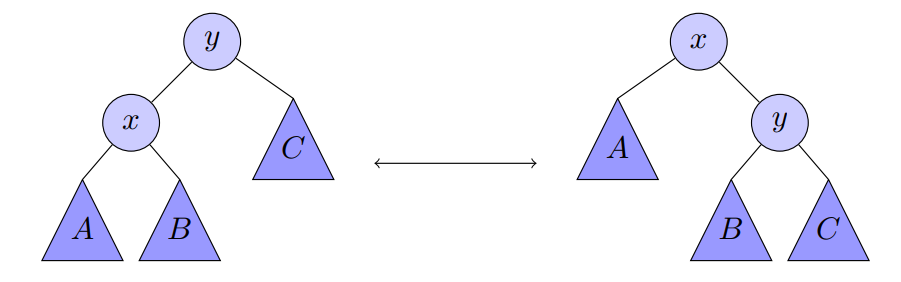
\includegraphics[width=0.7\textwidth]{../images/rotationExplication.png}\\[-0.5cm]
\end{center}

Une telle rotation préserve la propriété d'arbre binaire mais permet de rétablir la propriété de tas. Désormais pour insérer un noeud \( z \) dans un arbre 
    cartésien, il sera inséré comme dans un arbre binaire de recherche mais une fois cela effectué, tant que sa priorité est inférieure à celle de son noeud 
    parent, effectuer une rotation au noeud \( z \). Chaque rotation diminue la profondeur du noeud \( z \) de 1 et augmente celle de son parent de 1. 
    Les rotations peuvent être effectuées en temps constant puisqu'il s'agit simplement de manipulation de pointeurs.

\vspace{2cm}

\addcontentsline{toc}{section}{b. Complexité de l'algorithme d'insertion}

\textbf{3.b]} Donnez la complexité de cet algorithme en fonction de la profondeur de son prédécesseur.



\begin{tcolorbox}[colback=gray!10, colframe=blue!30, coltitle=black, title=Réponse à la 3.b - 1/2]

    L'insertion dans un arbre cartésien suit deux étapes :\\[-0.4cm]
    \begin{itemize}
        \item L'insertion classique dans un arbre binaire de recherche.
        \item La succession de rotations jusqu'à que la propriété du tas soit respectée.
    \end{itemize}

    \vspace{0.5cm}
    \hrule
    \vspace{0.5cm}

    Posons \( x \) le noeud à insérer.\\

    L'insertion d'un noeud dans un ABR consiste à une suite de comparaison pour rechercher la future place de ce dernier, en respectant l'ordre des clés. 
        Comme pour son algorithme de recherche, son insertion repose sur le nombre de comparaisons nécessaires pour trouver la position du nouveau noeud, 
        alias \( d(x) \) la profondeur du noeud inséré.\\

    Donc pour la première étape, l'insertion classique d'un ABR a une complexité de \( O(d(x)) \).

\end{tcolorbox}
\begin{tcolorbox}[colback=gray!10, colframe=blue!30, coltitle=black, title=Réponse à la 3.b - 2/2]

    La seconde étape consiste à une succession de rotations jusqu'à que la propriété du tas soit respectée. Ces rotations n'affectent en rien la propriété 
        des ABR. A chaque rotation, la profondeur du noeud inséré diminuera de 1. On recommence cette étape jusqu'à que la propriété du tas soit respectée.\\

    Dans le pire des cas, nous devons remonter le noeud jusqu'à la racine, on aura donc \( d(x) \) rotations à faire car on le remonte d'un seul niveau par 
        rotation. C'est le nombre maximal de rotations.\\

    Etant donné que chaque rotation se fait en temps constant, la complexité totale des rotations est en \( O(d(x)) \).\\[-0.4cm]

    \vspace{0.5cm}
    \hrule
    \vspace{0.5cm}

    La complexité totale de l'insertion dans un arbre cartésien est donc de :
    \[
    \ O(d(x)) + O(d(x)) = O(d(x))
    \]

    \vspace{0.5cm}
    \hrule
    \vspace{0.5cm}

    En conclusion, pour les mêmes raisons qu'en 2.b, on aura comme complexité pour un arbre cartésien à \( n \) noeuds :
    \begin{itemize}
        \item \textbf{S'il est équilibré :} \( O(\log n) \)
        \item \textbf{S'il est déséquilibré :} \( O(n) \)
    \end{itemize}

\end{tcolorbox}



%--------------------------------------------------------------------------------
% Question 3.c
%--------------------------------------------------------------------------------

\newpage
\addcontentsline{toc}{section}{c. Implantation de l'algorithme d'insertion}

\textbf{3.b]} Implanter cet algorithme.



\begin{tcolorbox}[colback=gray!10, colframe=blue!30, coltitle=black, title=Réponse à la 3.c - 1/1]

    Les méthodes \texttt{insert} et \texttt{insertRec} dans le fichier \href{./src/CartesianTree.java}{./src/CartesianTree.java} correspondent à 
        l'implantation de l'algorithme d'insertion de noeud. (l.95-136)

\end{tcolorbox}



%--------------------------------------------------------------------------------
% Question 3.d
%--------------------------------------------------------------------------------

\vspace{1.5cm}
\addcontentsline{toc}{section}{d. Tests d'insertion de noeuds}

\textbf{3.d]} Appliquer votre algorithme pour créer les arbres cartésiens obtenus en insérant les noeuds suivant dans l'ordre donné :
\begin{enumerate}
    \item (A:5), (B:3), (C:8), (D:2), (E:6), (F:7), (G:6), (H:1), (I:10), (J:12)
    \item (H:1), (G:9), (A:5), (B:3), (D:2), (F:7), (C:8), (J:12), (I:10), (E:6)
    \item (E:6), (H:1), (B:3), (D:2), (C:8), (F:7), (G:9), (J:12), (A:5), (I:10)
\end{enumerate}
et vérifier que vous obtenez bien à chaque fois le même arbre cartésien que dans la question \textbf{1.a.}



\begin{tcolorbox}[colback=gray!10, colframe=blue!30, coltitle=black, title=Réponse à la 3.d - 1/1]

    Les tests d'insertion se trouvent dans le fichier test : \href{./test/Exo\_3\_d.java}{./test/Exo\_3\_d.java}\\

    Chaque test vérifie que l'arbre obtenu est bien celui de la question \textbf{1.a} grâce à la méthode \texttt{equals} qui teste si un arbre est égal 
        à un autre (selon les clés). De plus, chaque arbre est affiché dans la console de débogage. 

\end{tcolorbox}





%--------------------------------------------------------------------------------
% Exercice 4 : Suppression dans un arbre cartésien
%--------------------------------------------------------------------------------

\newpage

\renewcommand{\chaptername}{Exercice}
\chapter{Suppression dans un arbre cartésien}



%--------------------------------------------------------------------------------
% Question 4.a
%--------------------------------------------------------------------------------

\addcontentsline{toc}{section}{a. Explication de la suppression de noeuds par rotation}

\textbf{4.a]} Expliquer pourquoi pour supprimer un noeud \( z \) dans un arbre cartésien, il est possible de faire des rotations dans l'autre sens avec son 
    fils qui a la priorité la plus faible jusqu'à l'amener à une feuille de l'arbre où il peut être supprimer. Chaque rotation augmente alors la profondeur
    du noeud \( z \) de 1 et diminue celle de son fils qui a la priorité la plus faible de 1. 



\begin{tcolorbox}[colback=gray!10, colframe=blue!30, coltitle=black, title=Réponse à la 4.a - 1/1]

    Pour commencer, nous savons que les rotations préservent la propriété d'un ABR.

    \vspace{0.5cm}
    \hrule
    \vspace{0.5cm}

    Posons \( z \) le noeud à supprimer et \( x \) son fils qui a la priorité la plus faible. Nous souhaitons descendre \( z \) de l'arbre 
        jusqu'à qu'il devienne une feuille, et donc qu'on puisse le supprimer. Pour ça, nous pouvons déjà rechercher le noeud, et ensuite nous ferons une 
        suite de rotations dans l'autre sens avec \( x \), jusqu'à qu'il devienne une feuille.\\

    Nous pouvons facilement constater que chaque rotation ne violera pas la propriété du tas (sans compter \( z \)), en effet :\\[-0.4cm]
    \begin{itemize}

        \item \( x \) aura comme sous-noeuds : \( z \), son frère initial et ses enfants, ainsi que ses enfants initiaux.
        \item Étant donné qu'on cherche à supprimer \( z \), on ne le considère pas pour la propriété du tas.
        \item \( x \) était le fils de \( z \) avec la priorité la plus basse, il respecte donc la propriété du tas avec son frère initial, qui est maintenant à 
            un niveau inférieur. C'est également le cas avec les enfants du frère, qui ont une plus grande priorité que ce dernier.
        \item \( x \) a une priorité inférieure à ses enfants initiaux d'après l'arbre cartésien pré-rotation.

    \end{itemize}

    \vspace{0.5cm}
    \hrule
    \vspace{0.5cm}

    En répétant ce processus, nous finirons bien avec \( z \) qui deviendra une feuille, vu qu'il perd petit à petit son lien avec ses enfants à chaque rotation.
        Et enfin, nous pourrons le supprimer, tout en respectant les propriétés d'un arbre cartésien à la fin.


\end{tcolorbox}



%--------------------------------------------------------------------------------
% Question 4.b
%--------------------------------------------------------------------------------

\newpage
\addcontentsline{toc}{section}{b. Complexité de l'algorithme de suppression de noeud}

\textbf{4.b]} Donner la complexité de l'algorithme obtenu.



\begin{tcolorbox}[colback=gray!10, colframe=blue!30, coltitle=black, title=Réponse à la 4.b - 1/1]

    L'algorithme de suppression dans un arbre cartésien se fait en deux étapes :\\[-0.4cm]
    \begin{itemize}
        \item La recherche du noeud à supprimer.
        \item Une suite de rotation du noeud à supprimer, jusqu'au fond de l'arbre.
    \end{itemize}

    \vspace{0.5cm}
    \hrule
    \vspace{0.5cm}

    Nous remarquons vite que nous parcourons l'arbre du haut vers le bas, jusqu'à tomber sur une feuille, et que chaque étape se fait en temps constant.\\[-0.4cm]
    \begin{itemize}
        \item Comparer la clé du noeud à supprimer avec le noeud courant : temps constant.
        \item S'il y a une rotation : temps constant.
    \end{itemize}

    \vspace{0.5cm}

    La complexité de l'algorithme sera donc la profondeur de la feuille \( x \) rencontrée, que ce soit le noeud à supprimer ou non \( \Rightarrow \Theta(d(x)) \).

    \vspace{0.5cm}
    \hrule
    \vspace{0.5cm}

    En conclusion, pour les mêmes raisons qu'en 2.b, on aura comme complexité pour un arbre cartésien à \( n \) noeuds :\\[-0.4cm]
    \begin{itemize}
        \item \textbf{S'il est équilibré :} \( \Theta(\log n) \)
        \item \textbf{S'il est déséquilibré :} \( \Theta(n) \)
    \end{itemize}

\end{tcolorbox}



%--------------------------------------------------------------------------------
% Question 4.c
%--------------------------------------------------------------------------------

\vspace{1.5cm}
\addcontentsline{toc}{section}{c. Implantation de l'algorithme de suppression de noeud}

\textbf{4.c]} Implanter cet algorithme.



\begin{tcolorbox}[colback=gray!10, colframe=blue!30, coltitle=black, title=Réponse à la 4.c - 1/1]

    Les méthodes \texttt{delete} et \texttt{deleteRec} dans le fichier \href{./src/CartesianTree.java}{./src/CartesianTree.java} correspondent à 
        l'implantation de l'algorithme de suppression de noeud. (l.195-252)

\end{tcolorbox}



%--------------------------------------------------------------------------------
% Question 4.d
%--------------------------------------------------------------------------------

\vspace{1.5cm}
\addcontentsline{toc}{section}{d. Tests de suppression de noeuds}

\textbf{4.d]} Appliquer votre algorithme pour créer des arbres cartésiens obtenus en supprimant successivement les noeuds suivants dans l'arbre cartésien
    de la question \textbf{1.a} :

\[
\ (A:5), (J:12), (H:1)
\]



\begin{tcolorbox}[colback=gray!10, colframe=blue!30, coltitle=black, title=Réponse à la 4.d - 1/1]

    Les tests d'insertion se trouvent dans le fichier test : \href{./test/Exo\_4\_d.java}{./test/Exo\_4\_d.java}\\

    Chaque test vérifie que l'arbre obtenu après suppression est correct grâce à la méthode \texttt{equals}. En effet, on construit également
        un arbre avec les insertions SANS le noeud supprimé à côté. De plus, après chaque suppression, l'arbre est affiché dans la console
        de débogage.

\end{tcolorbox}





%--------------------------------------------------------------------------------
% Exercice 5 : Priorités aléatoires - Aspect expérimental
%--------------------------------------------------------------------------------

\newpage

\renewcommand{\chaptername}{Exercice}
\chapter{Priorités aléatoires - Aspect expérimental}

Un arbre cartésien \textit{aléatoire} est un arbre dans lequel les priorités sont tirés uniformément aléatoirement dans l'intervalle [0,1]. Il est possible
    d'utiliser des entiers dans un intervalle suffisamment grand pour espérer que tous les noeuds auront des clés différentes avec une très forte probabilité.\\

Pour insérer une nouvelle clé dans un arbre cartésien aléatoire, une priorité est itrée uniformément aléatoirement et c'est le noeud formé de cette clé et de
    cette priorité qui est inséré dans l'arbre.



%--------------------------------------------------------------------------------
% Question 5.a
%--------------------------------------------------------------------------------

Effectuer une analyse très détaillée d'efficacité expérimentale de votre structure de données pour un tel arbre cartésien aléatoire. En particulier :\\[-0.4cm]
\begin{itemize}
    \item expliquer quelles métriques sont pertinentes pour évaluer l'équilibre et l'efficacité d'un arbre cartésien par rapport à d'autres structures de données;
    \item faire une analyse de ces métriques sur des arbres cartésiens avec un nombre de noeuds le plus grand possible (pour votre implantation);
    \item donner un exemple d'une séquence d'insertion qui pourrait déséquilibrer un arbre binaire de recherche classique et expliquez comment un arbre cartésien se défend
        contre cela grâce à sa structure aléatoire;
    \item discuter, le cas échéant, des implications de la collision des priorités sur la structure de l'arbre et sur les performances des opérations.
\end{itemize}

\vspace{0.5cm}

%--------------------------------------------------------------------------------
% Les métriques pertinentes
%--------------------------------------------------------------------------------

\addcontentsline{toc}{section}{a. Les métriques pertinentes}
\begin{tcolorbox}[colback=gray!10, colframe=blue!30, coltitle=black, title=Les métriques pertinentes]

    Afin d'évaluer l'équilibre et l'efficacité d'un arbre cartésien par rapport à d'autres structures de données, on utilisera les métriques suivantes :

    \begin{itemize}
        \item \textbf{La profondeur moyenne et maximale :} En effet, ces derniers reflettent l'équilibre d'un arbre, et aura forcément un coup sur la complexité de certaines
            opérations. Il est donc important de les comparer avec les autres structures.
        \item \textbf{Le temps d'exécution :} Il faut comparer le temps de recherche, d'insertion et de suppression de notre arbre cartésien aléatoire et des autres
            structures de données.
        \item \textbf{Comparaison avec des structures de données équilibrées} : Nous allons comparer les métriques précédentes en utilisant les AVL et les arbres 
            rouge-noir, qui donnent des arbres équilibrés. Si les résultats sont "proches", alors notre arbre cartésien aléatoire est intéressante, et naturellement
            presque équilibrée.
    \end{itemize}

\end{tcolorbox}

\newpage

%--------------------------------------------------------------------------------
% L'analyse des métriques
%--------------------------------------------------------------------------------

\addcontentsline{toc}{section}{a. Analyse des métriques}
\begin{tcolorbox}[colback=gray!10, colframe=blue!30, coltitle=black, title=Analyse des métriques - 1/2]

    Après avoir exécuté \href{./src/Experimentation\_CartesienTreeRandom.java}{./src/Experimentation\_CartesienTreeRandom.java} plusieurs fois, et pour des \( n \) différents,
        voici une moyenne des résultats :\\

    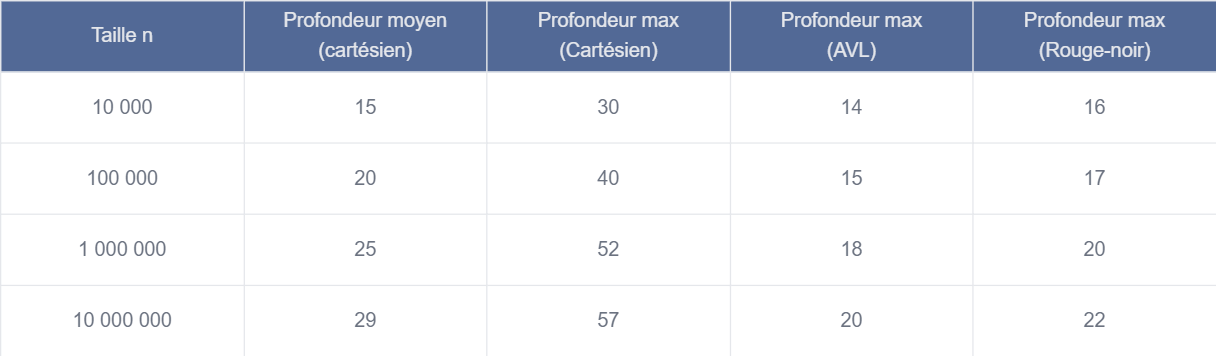
\includegraphics[width=1\textwidth]{../images/profondeur.png}\\
    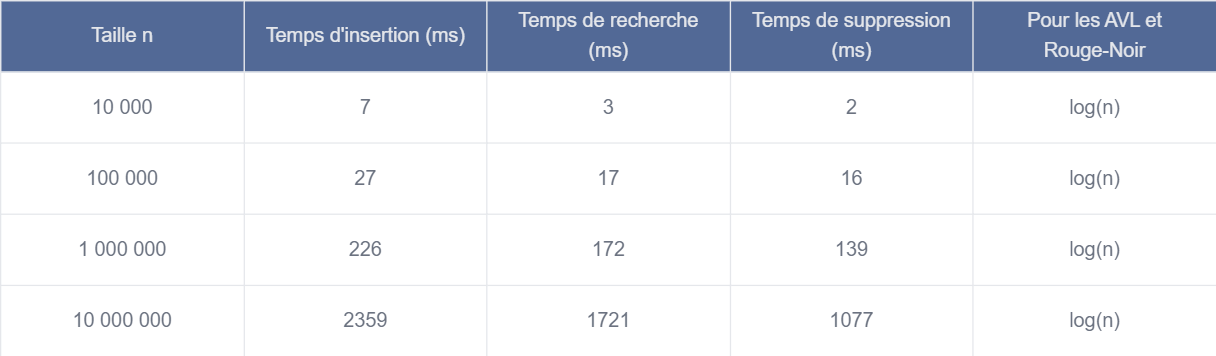
\includegraphics[width=1\textwidth]{../images/temps.png}

    \vspace{0.5cm}
    \hrule
    \vspace{0.5cm}

    Pour commencer, nous voyons bien que la profondeur moyenne est proche de \( O(log n) \). En effet, en faisant pour chacune des profondeurs moyennes des arbres cartésien
        \( \log_2(n) \), nous aurons un peu près les mêmes valeurs. Par exemple, \( \log_2(10000) = 13\), ce qui est proche de 15.\\

    Pour les profondeurs max, il est normal qu'ils soient supérieures à ceux des autres structures de données équilibrées. En effet, dû à la nature probabiliste 
        des priorités, il se peut que certaines sous-arbres soient déséquilibrés. Mais les résultats restent satisfaisants.

\end{tcolorbox}
\begin{tcolorbox}[colback=gray!10, colframe=blue!30, coltitle=black, title=Analyse des métriques - 2/2]

    Pour les temps d'exécution des opérations insertion, recherche et suppression, ceux des arbres équilibrées VL et Rouge-Noir sont de l'ordre de \( O(\log n) \).\\
    
    L'arbre cartésien nous montre que les résultats croit de manière significative avec \( n \), mais ça reste plus lent que \( n \) lui-même, et les valeurs de temps
        sont relativement proportionnelle à \( \log n \). \\
    
    On peut le vérifier une dernière fois avec la différence de croissance de temps.\\[-0.4cm]
    \begin{itemize}
        \item \textbf{Croissance des log pour chaque n} : \(\log(10000) = 4\), \(\log(100000) = 5\), \(\log(1000000) = 6\), \(\log(10000000) = 7\)\\[-0.3cm]
        \item \textbf{Croissance du temps d'insertion } :
        \begin{itemize}
            \item \textbf{Entre n = 10000 et 100000} : \( 20 \) ms (insertion), \( 14 \) ms (recherche), \( 14 \) ms (suppression).
            \item \textbf{Entre n = 100000 et 1000000} : \( 199 \) ms (insertion), \( 155 \) ms (recherche), \( 120 \) ms (suppression).
            \item \textbf{Entre n = 1000000 et 10000000} : \( 2130 \) ms (insertion), \( 1549 \) ms (recherche), \( 938 \) ms (suppression).
        \end{itemize}
    \end{itemize}

    \vspace{0.5cm}

    Les différences sont significatives, certes, mais on voit qu'ils suivent la tendance d'augmentation des temps qui est proportionnelle à \( \log(n) \).

    \vspace{0.5cm}
    \hrule
    \vspace{0.5cm}

    En conclusion, pour des \( n \) de plus en plus grand, notre arbre cartésien aléatoire deviendra naturellement équilibré, permettant donc d'avoir une 
        complexité d'insertion, de recherche et de suppression optimale. Bien évidemment, à cause de l'aléatoire, nous pouvons tomber sur des cas où les performances 
        sont moindres, voir dans les cas extrêmes, d'avoir un arbre déséquilibré. Mais cela reste de plus en plus rare, quand \( n \) augmente.

\end{tcolorbox}

\newpage

%--------------------------------------------------------------------------------
% La défense de l'arbre cartésien aléatoire face à l'arbre binaire de recherche
%--------------------------------------------------------------------------------

\addcontentsline{toc}{section}{a. La défense de l'arbre cartésien aléatoire face à l'arbre binaire de recherche}
\begin{tcolorbox}[colback=gray!10, colframe=blue!30, coltitle=black, title=La défense de l'arbre cartésien aléatoire face à l'arbre binaire de recherche - 1/1]

    Prenons une insertion où chaque nouvelle clé insérée est forcément supérieure à celles précédentes. Dans la logique d'insertion d'un arbre binaire de recherche,
        nous finirons sur un arbre totalement déséquilibré qui représentera plus une chaîne qu'un arbre.\\

    Grâce à la structure aléatoire de notre arbre cartésien classique, on garde l'avantage d'un arbre binaire de recherche avec les clés... Mais aussi d'éviter le plus
        possible le cas d'une suite d'insertion non-avantageuse. En effet, en attribuant au hasard des priorités à ces éléments, l'ordre d'insertion devient négligeable,
        étant donné que la priorité dicte la hauteur des noeuds. \\
        
    De plus, nous avons vu plus haut que la nature aléatoire des priorités permettent d'avoir un équilibre
        probable, quoi que leurs clés soient triés ou non. Nous pouvons le vérifier avec notre code, où nous avons inséré constamment une clé supérieure après une autre.\\

    En conclusion, un arbre cartsien se défend bien face à ce genre de séquence d'insertion en rendant uniformément aléatoire la priorité des noeuds, permettant ainsi
        d'avoir une très faible chance d'avoir un arbre totalement déséquilibré.

\end{tcolorbox}

\vspace{0.5cm}
\hrule
\vspace{0.5cm}

%--------------------------------------------------------------------------------
% La collision des priorités et les performances des opérations
%--------------------------------------------------------------------------------

\addcontentsline{toc}{section}{a. La collision des priorités et les performances des opérations}
\begin{tcolorbox}[colback=gray!10, colframe=blue!30, coltitle=black, title=La collision des priorités et les performances des opérations - 1/1]

    Dans le cas rare mais possible qu'on tombe sur des noeuds ayant les mêmes priorités, alors nous pouvons avoir plusieurs soucis.\\
    
    Par exemple, dans \textbf{l'ordre d'insertion}, la stratégie implantée est ambigue. On ne sait pas quelle noeud doit être le parent de l'autre. Par conséquent, cela 
        pourrait s'avérer être du hasard, et nous pourrions voir le risque d'avoir un arbre totalement déséquilibré. Et forcément, les performances des opérations 
        seraient négativement impactées, étant donné qu'elles reposent sur les profondeurs des noeuds.\\

    Les collisions des priorités peut donc devenir un grave soucis pour la complexité des opérations, et pour l'équilibre de l'arbre. Dans le cas de l'arbre cartésien
        aléatoire, il est certes possible d'en avoir, mais si nous choisissons nos clés uniformément aléatoirement dans un intervalle suffisamment grand, alors il
        reste très peu probable que ça arrive. Les bienfaits de cette structure surclasse donc l'inconvénient des collisions des priorités, et reste intéressante comme
        alternatives.

\end{tcolorbox}





%--------------------------------------------------------------------------------
% Exercice 6 : Priorités aléatoires - Aspect théorique
%--------------------------------------------------------------------------------

\newpage

\renewcommand{\chaptername}{Exercice}
\chapter{Priorités aléatoires - Aspect théorique}

L'objectif de cet exercice est de démontrer que la profondeur moyenne d'un noeud d'un arbre cartésien à n noeuds est en \( O(\log n) \). Considérons un tel
    arbre et \( x_k \) le noeud dont la clé est la \( k \)-ième plus petite de l'arbre. Notons \( X_{ik} \) la variable aléatoire indiquant que \( x_i \) est
    un ancêtre propre de \( x_k \) (pour le tirage aléatoire des priorités).



%--------------------------------------------------------------------------------
% Question 6.a
%--------------------------------------------------------------------------------

\vspace{1.5cm}
\addcontentsline{toc}{section}{a. Profondeur moyenne de \( x_k \)}

\textbf{6.a]} Montrer que la profondeur moyenne de \( x_k \) est égale à \(\sum_{i = 1}^{n} \mathbb{E}[X_{ik}]\).



\begin{tcolorbox}[colback=gray!10, colframe=blue!30, coltitle=black, title=Réponse à la 6.a - 1/2]

    Pour commencer, nous devons trouver une formulation pour exprimer la profondeur de \( x_k \) dans un arbre cartésien.

    \vspace{0.5cm}
    \hrule
    \vspace{0.5cm}

    La profondeur d'un noeud \( x_k \) noté \( d(x_k) \) dans un arbre représente le nombre d'arêtes qu'on doit traverser de la racine jusqu'à \( x_k \). Autrement dit,
        sa profondeur représente le nombre d'ancêtre propre qu'il possède.\\

    Par conséquent, si on définie la variable aléatoire \( X_{ik} \) de la manière suivante :
    \[
    \ X_{ik} =
    \begin{cases}
        1 \text{ si \(x_i\) est un ancêtre de \(x_k\).} \\
        0 \text{ sinon.}
    \end{cases}
    \]

    \vspace{0.5cm}

    Alors nous pouvons formuler la profondeur de \( x_k \) comme :
    \[
    \ d(x_k) = \sum_{i=1}^{n} X_{ik}
    \]

    \vspace{0.5cm}
    \hrule
    \vspace{0.5cm}

    La moyenne des profondeurs de \( x_k \) correspond à l'espérance de cette formule :
    \[
    \ d_{moy}(x_k) = \mathbb{E}[\sum_{i = 1}^{n} X_{ik}]
    \]

\end{tcolorbox}
\begin{tcolorbox}[colback=gray!10, colframe=blue!30, coltitle=black, title=Réponse à la 6.a - 2/2]

    Or, d'après la linéarisation de l'espérance, c'est-à-dire \( \mathbb{E}[a+b] = \mathbb{E}[a] + \mathbb{E}[b] \), on a donc :
    \[
    \ d_{moy}(x_k) = \mathbb{E}[\sum_{i = 1}^{n} X_{ik}] = \sum_{i = 1}^{n} \mathbb{E}[X_{ik}]
    \]

    \vspace{0.5cm}
    \hrule
    \vspace{0.5cm}

    En conclusion, nous avons démontré que la profondeur moyenne de \( x_k \) est égale à \(\sum_{i = 1}^{n} \mathbb{E}[X_{ik}]\).

\end{tcolorbox}  



%--------------------------------------------------------------------------------
% Question 6.b
%--------------------------------------------------------------------------------

\newpage
\addcontentsline{toc}{section}{b. Relation entre \( X(i,k) \) et \( X_{ik} \)}

\textbf{6.b]} Notons \( X(i,k) \) l'ensemble des noeuds \( \{x_i, x_{i+1}, \dots, x_k \} \) ou \( \{x_k, x_{k+1}, \dots, x_i \} \) suivant selon \(i < k\) 
    ou \( i > k \). Montrer que \( X_{ik} = 1 \) si et seulement si \( x_i \) est le noeud qui a la plus petite priorité dans \( X(i,k) \).



\begin{tcolorbox}[colback=gray!10, colframe=blue!30, coltitle=black, title=Réponse à la 6.b - 1/1]

    Prouvons que \( X_{ik} = 1 \Longleftrightarrow x_i \) est le noeud ayant la priorité minimale dans \( X(i,k) \).

    \vspace{0.5cm}
    \hrule
    \vspace{0.5cm}

    Supposons que \( X_{ik} = 1 \). \( x_i \) est donc un ancêtre propre de \( x_k \).\\

    Nous savons que \( x_i \) appartient à l'ensemble \( X(i,k) \), qui par définition, représente tous les noeuds entre \( x_i \) et \( x_k \) dans
        l'ordre des clés.\\[-0.4cm]
    \begin{itemize}
        \item Vu que \( x_i \) est un ancêtre propre de \( x_k \), alors sa priorité est forcément plus faible.
    \end{itemize}

    \vspace{0.5cm}

    Supposons par l'absurde qu'un noeud \( x_j \) tel que (\( i < j < k \)) ou (\( i > j > k \)) possède une priorité plus faible que \( x_i \).\\[-0.4cm]
    \begin{itemize}
        \item \textbf{D'après la propriété du tas :} \( x_j \) serait au dessus de \( x_i \) et de \( x_k \).
        \item \textbf{D'après la propriété d'un ABR :} étant donné qu'on a les clés (\( i < j < k \)) ou (\( i > j > k \)), alors \( x_i \) et \( x_k \) ne peuvent pas être dans
            le même sous-arbre de \( x_j \), ce qui est en contradiction avec notre hypothèse, \( x_i \) ne pourrait pas être un ancêtre propre de \( x_k \).
    \end{itemize}

    \vspace{0.5cm}

    Donc en supposant que \( X_{ik} = 1 \), \( x_i \) doit forcément avoir la priorité la plus faible de l'ensemble \( X(i,k) \), sinon il y aurait une 
        contradiction.

    \vspace{0.5cm}
    \hrule
    \vspace{0.5cm}

    Supposons que \( x_i \) est le noeud ayant la priorité minimale dans \( X(i,k) \).\\

    Nous pouvons déduire que \( x_i \) est un ancêtre propre de \( x_k \) grâce à ces propriétés :\\[-0.4cm]
    \begin{itemize}
        \item \textbf{D'après la propriété du tas :} \( x_i \) est au dessus de tous les autres noeuds de \( X(i,k) \), \( x_k \) compris.
        \item \textbf{D'après la propriété d'un ABR :} Etant donné que les clés de \( x_i \) et \( x_k \) délimitent \( X(i,k) \), alors \( x_k \) est 
            forcément dans un des sous-arbre de \( x_i \).
    \end{itemize}

    \vspace{0.5cm}

    Donc en supposant que \( x_i \) est le noeud ayant la priorité minimale dans \( X(i,k) \), on a démontré que \( x_i \) est un ancêtre propre de \( x_k \),
        donc que \( X_{ik} = 1\).

    \vspace{0.5cm}
    \hrule
    \vspace{0.5cm}

    Nous avons donc bien démontré que \( X_{ik} = 1 \) si et seulement si \( x_i \) est le noeud qui a la plus petite priorité dans \( X(i,k) \)

\end{tcolorbox}



%--------------------------------------------------------------------------------
% Question 6.c
%--------------------------------------------------------------------------------

\newpage
\addcontentsline{toc}{section}{c. Conclusion}

\textbf{6.c]} Conclure (en vous inspirant de la preuve de la complexité en moyenne du tri rapide vue en cours).



\begin{tcolorbox}[colback=gray!10, colframe=blue!30, coltitle=black, title=Réponse à la 6.c - 1/3]

    Pour rappel, nous savons que :\\[-0.4cm]
    \begin{itemize}
        \item la profondeur moyenne de \( x_k \) est égale à \(\sum_{i = 1}^{n} \mathbb{E}[X_{ik}]\).
        \item \( X_{ik} = 1 \) si et seulement si \( x_i \) est le noeud qui a la plus petite priorité dans \( X(i,k) \).
    \end{itemize}

    Et on suppose que toutes les priorités sont différentes.

    \vspace{0.5cm}
    \hrule
    \vspace{0.5cm}

    On sait que \( X_{ik} = 1 \Longleftrightarrow x_i \) est le noeud ayant la priorité minimale dans \( X(i,k) \) et que les priorités de tous les noeuds sont 
        tiré uniformément aléatoirement, par conséquent :\\[-0.4cm]
    \begin{itemize}
        \item \textbf{Grâce à la réciproque :} on peut déduire que la probabilité que \( X_{i,k} = 1 \) est égale à la probabilité que \( x_i \) possède la plus faible
            priorité dans \(X(i,k)\), donc une chance sur tous les noeuds présents.
        \item \textbf{Grâce à l'uniformité de l'aléatoire :} on peut déduire que l'espérance de \( X_{ik} \) est égale à la probabilité que \( X_{i,k} = 1 \).
    \end{itemize}
        
    \[
    \ \mathbb{E}[X_{ik}] = P(X_{ik} = 1) = \frac{1}{|X(i,k)|}
    \] 

    \vspace{0.5cm}

    De plus, nous pouvons facilement déduire que \( |X(i,k)| = | i - k + 1 | \) noeuds, ou autrement dit :
    \[
    \ |X(i,k)| =
    \begin{cases}
        i - k + 1 \text{ noeuds \quad si i > k} \\
        k - i + 1 \text{ noeuds \quad si i < k} 
    \end{cases}
    \]

    \vspace{0.5cm}

    Le cas \( i = k \) n'est pas défini pour X(i,k), on l'ignorera donc.

    \vspace{0.5cm}
    \hrule
    \vspace{0.5cm}

    Nous savons que la profondeur moyenne de \( x_k \) est égale à \(\sum_{i \in {1, \dots, n} \ } \mathbb{E}[X_{ik}]\). Par conséquent, nous avons :
    \[
    \ d_{moy}(x_k) = \sum_{i = 1}^{n} \mathbb{E}[X_{ik}] = \sum_{i \in \{1, \dots, n\} \textbackslash \{k\}} \frac{1}{|i - k| + 1}
    \]

    \vspace{0.5cm}

    On peut donc le réécrire de cette manière :
    \[
    \ d_{moy}(x_k) = \sum_{i = 1}^{k-1} \frac{1}{k - i + 1} + \sum_{i = k+1}^{n} \frac{1}{i - k + 1}
    \]

    \vspace{0.5cm}

    Et avec un changement de variable où l'on pose \( j = k - i \):
    \[
    \ d_{moy}(x_k) = \sum_{j = 1}^{k-1} \frac{1}{j + 1} + \sum_{j = k+1}^{n - k} \frac{1}{j + 1}
    \]

\end{tcolorbox}
\begin{tcolorbox}[colback=gray!10, colframe=blue!30, coltitle=black, title=Réponse à la 6.c - 2/3]

    En cours, nous avons vu la preuve de la complexité en moyenne du tri rapide, qui comportait une partie sur les nombres harmoniques. On s'inspirera de cette dernière.\\

    \vspace{0.5cm}
    \hrule
    \vspace{0.5cm}

    Pour la première somme de la formule que l'on notera \( S_1 \), nous avons :
    \[
    \ S_1 = \frac{1}{2} + \frac{1}{3} + \dots + \frac{1}{k-1} = \sum_{j = 1}^{k-1} \frac{1}{j + 1}
    \]

    \vspace{0.5cm}

    Nous avons donc :
    \[
    \ \int_{j}^{j+1} \frac{1}{t+1} \; dt \leq \frac{1}{j+1} \leq \int_{j-1}^{j} \frac{1}{t+1} \; dt
    \]

    \vspace{0.5cm}

    En sommant de 1 à \( k-1 \) :
    \[
    \ \int_{1}^{k} \frac{1}{t+1} \; dt \leq S_1 \leq 1 + \int_{1}^{k-1} \frac{1}{t+1} \; dt
    \]

    \vspace{0.5cm}

    Donc :
    \[
    \ \ln(k+1) - \ln(2) \leq S_1 \leq 1 + (\ln(k) - \ln(2)) \quad \text{ et } \quad S_1 \sim \ln(k)
    \]

    \vspace{0.5cm}
    \hrule
    \vspace{0.5cm}

    Pour la seconde somme de la formule que l'on notera \( S_2 \), nous avons :
    \[
    \ S_2 = \frac{1}{k+1} + \frac{1}{k+2} + \dots + \frac{1}{n-k} = \sum_{j = k+1}^{n-k} \frac{1}{j + 1}
    \]

    \vspace{0.5cm}

    Nous avons donc :
    \[
    \ \int_{j}^{j+1} \frac{1}{t+1} \; dt \leq \frac{1}{j+1} \leq \int_{j-1}^{j} \frac{1}{t+1} \; dt
    \]

    \vspace{0.5cm}

    En sommant de \( k+1 \) à \( n-k \) :
    \[
    \ \int_{k+1}^{n-k+1} \frac{1}{t+1} \; dt \leq S_2 \leq \int_{k}^{n-k} \frac{1}{t+1} \; dt
    \]

    \vspace{0.5cm}

    Donc :
    \[
    \ \ln(n - k + 2) - \ln(k + 2) \leq S_2 \leq \ln(n - k + 1) - \ln(k + 1) \quad \text{ et } \quad S_2 \sim \ln(\frac{n}{k})
    \]

\end{tcolorbox}
\begin{tcolorbox}[colback=gray!10, colframe=blue!30, coltitle=black, title=Réponse à la 6.c - 3/3]

    Nous avons réussi à donner une approximation aux deux sommes composant \(d_{moy}(x_k)\), nous pouvons lui aussi l'approcher :
    \[ d_{moy}(x_k) = S_1 + S_2 \sim \ln(k) + \ln(\frac{n}{k}) \]
    \[ d_{moy}(x_k) \sim \ln(k * \frac{n}{k}) \]
    \[ d_{moy}(x_k) \sim \ln(n) \]

    \vspace{0.5cm}
    \hrule
    \vspace{0.5cm}

    En conclusion, nous avons bel et bien démontré que la profondeur moyenne d'un noeud \( x_k \) d'un arbre cartésien à n noeuds est en \( O(\ln n)\), et 
        donc en \( O(\log n) \).

\end{tcolorbox}




\end{document}